% Chapter 5

\chapter{Results} % Main chapter title

\label{Chapter5}

%-------------------------------------------------------------------------------
%-------------------------------------------------------------------------------

\section{Results}\label{section:results}

Preliminary results show distinct patterns in the distribution of both Cohune Palm and deciduous trees. Our best results using YOLOv2 CNN to classify the individual trees resulted in an average precision (AP) of $79.5\%$ for Cohune Palm and $67.3\%$ AP for deciduous trees ~\ref{fig:PR-palm-deciduous-bfree} at the main BFREE site. Furthermore testing at our more distant sites: Oro and Ramos we scored an $67.1\%$ and $76.0\%$ AP on Cohune Palms and $64.9\%$ and $84.2\%$ AP on Deciduous trees respectively. See table ~\ref{table:ap-results} below. This shows that our network was able to generalize enough to more distant sites that had both lower resolution and different lighting conditions due to low hanging clouds.

\begin{center}
    \begin{table}[h]\footnotesize
        \caption{Average Precision for each site per class}\label{table:ap-results}
        \begin{tabular}{| l | l | l | l |}
        \hline
        Site & Resolution (cm/pixel) & Cohune Palm (AP) & Deciduous Trees (AP)\\ \hline
        BFREE & 4.93  & $79.5\%$ & $67.3\%$ \\
        Oro   & 10.95 & $67.1\%$ & $64.9\%$ \\
        Ramos & 10.60 & $76.0\%$ & $84.2\%$ \\
        \hline
        \end{tabular}
    \end{table}
\end{center}

For both Oro and Ramos the size of evaluation set of spiny trees is very small due to scarcity of deciduous trees in the labeled areas. Examining the outlier of Ramos spiny results revealed that the area labeled had a high number of easy detections as well leading to better then average results.

\begin{figure}[ht]
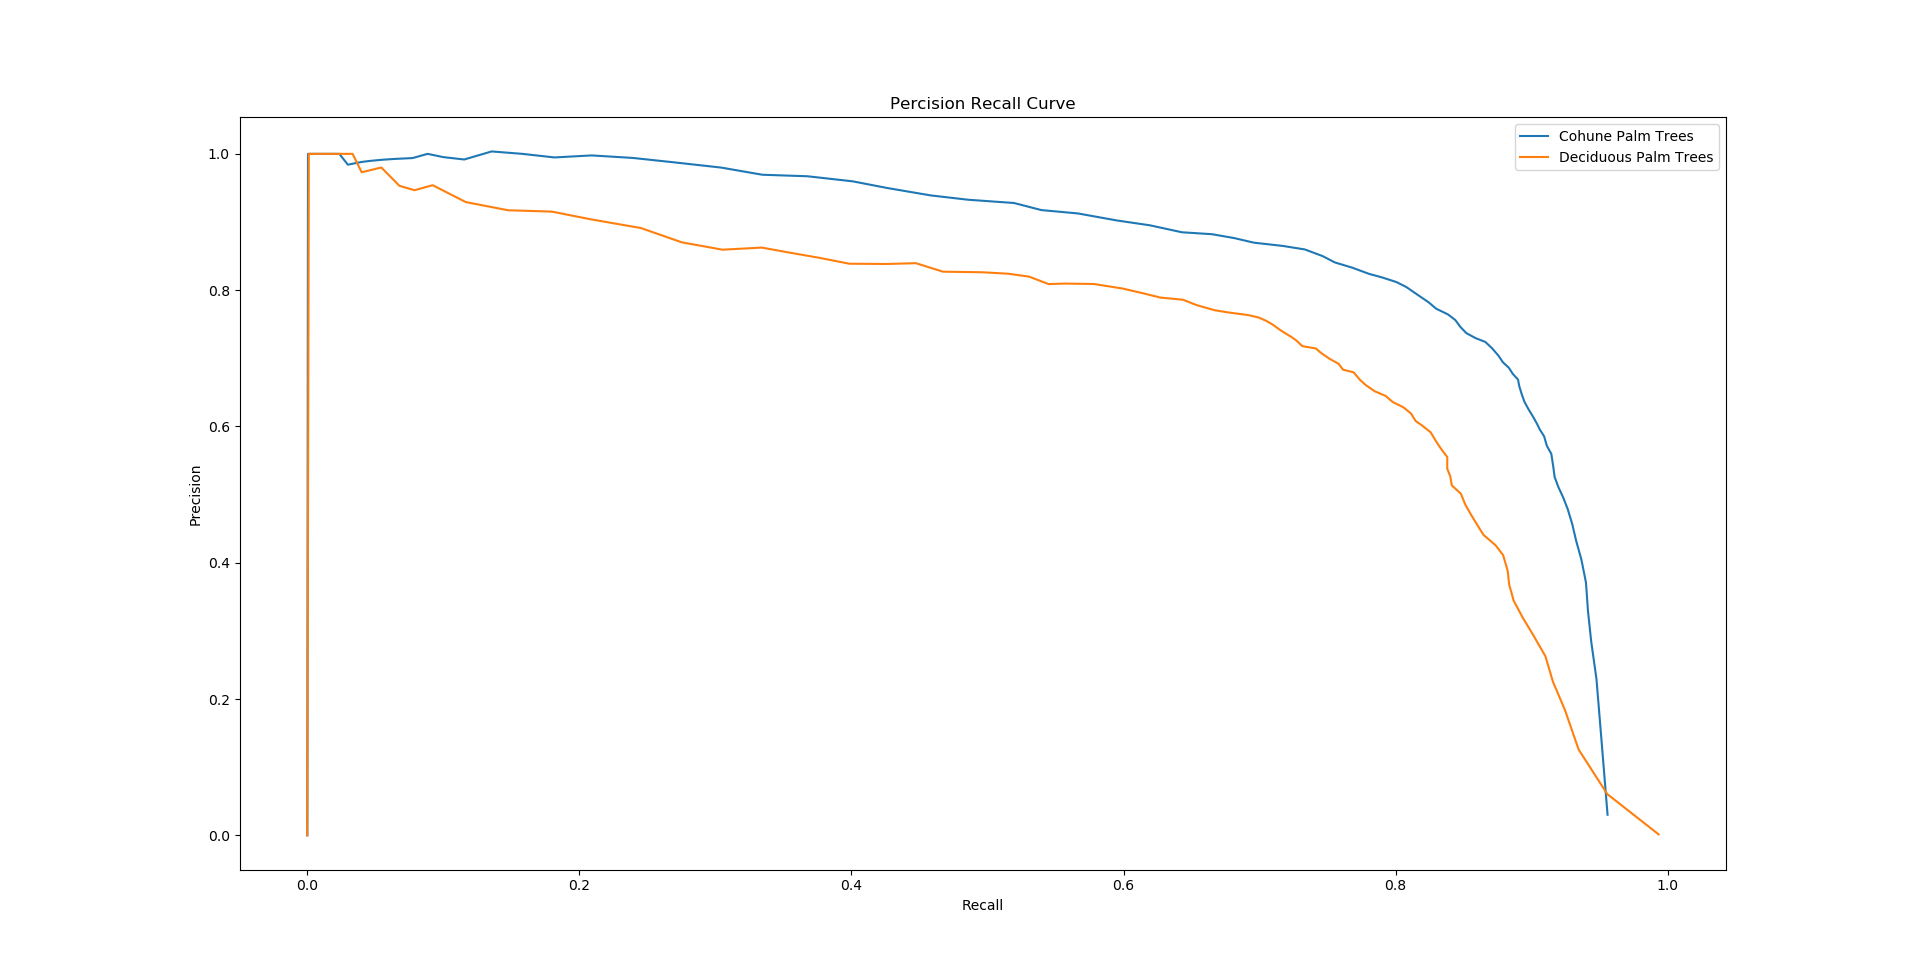
\includegraphics[width=1.0\textwidth]{Figures/PR-palm-deciduous-bfree.png}
\caption{Precision Recall for Cohune Palm Trees vs Deciduous Trees. We noticed a substantial intraclass difference with deciduous tree size and shape, correspondingly the network had a difficult time localizing individual trees with a high IOU.}
\label{fig:PR-palm-deciduous-bfree}
\end{figure}

\subsection{Effect of Network Resolution}

One aspect we explore in this work is the input resolution of the network. We found that it provided a mild boost of roughly $.8\%$ for our bfree site. However, it produced significantly better results for both Cohune Palm Trees and Deciduous trees of both Ramos and Oro. We hypthosize this is because the image resolution was already have of our main sites that any further down sampling to fit into the network input significantly hurt our performance.


\subsection{Effect of Image Resolution}

In ~\ref{fig:PR-resolution} we show the PR curves for various resolution of data starting for Cohune Palm trees starting from our base resolution of ~5 cm/pixel and going to 1m/pixel. The resolutions were artificially created by subsampling the original images as shown in Figure 11. Within the 5-20cm/pixel range we still have workable results; past 40 cm/pixel we seen a rapid decline. Typical satellite imagery lives in the range of 3 meters to 30 cm with the cost getting proportionally higher as resolution increases. We show with this technique that it is necessary to have very high resolution imagery in order to do fine grained species classification. More performance from the network might have been possible with greater tuning and training for lower resolution imagery; however, we believe that we are close to the upper limit. As the pictures in ~\ref{fig:Palm-resolution} show at a certain point the palm becomes indistinguishable to humans putting a bound on our ability to even create a dataset with which to train our network.

\begin{figure}[ht]
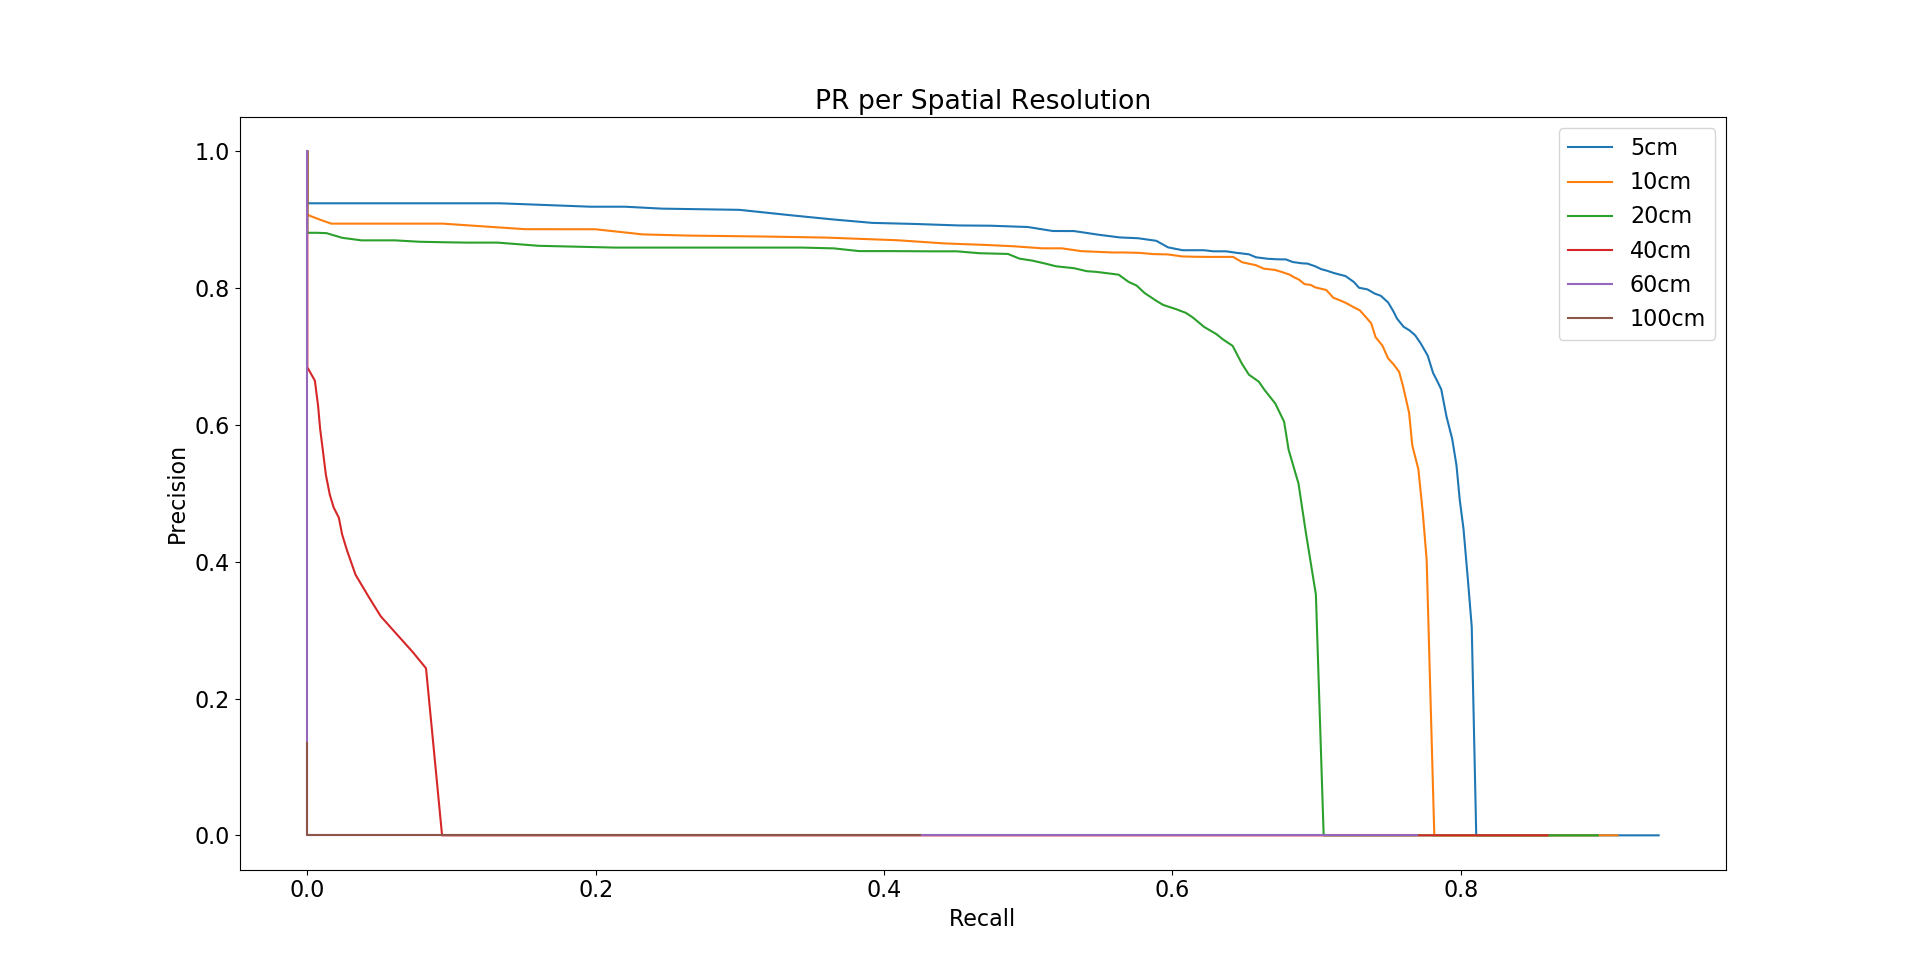
\includegraphics[width=1.0\textwidth]{Figures/PR-resolution.png}
\caption{Evaluating Precision Recall vs spatial resolution is important for planning future flights since gathering higher resolution requires flying at lower altitudes meaning you can cover less distance. Ideally we can find a sweet spot between image resolution and performance that lets us maximize area covered.}
\label{fig:PR-resolution}
\end{figure}

\begin{figure}[ht]
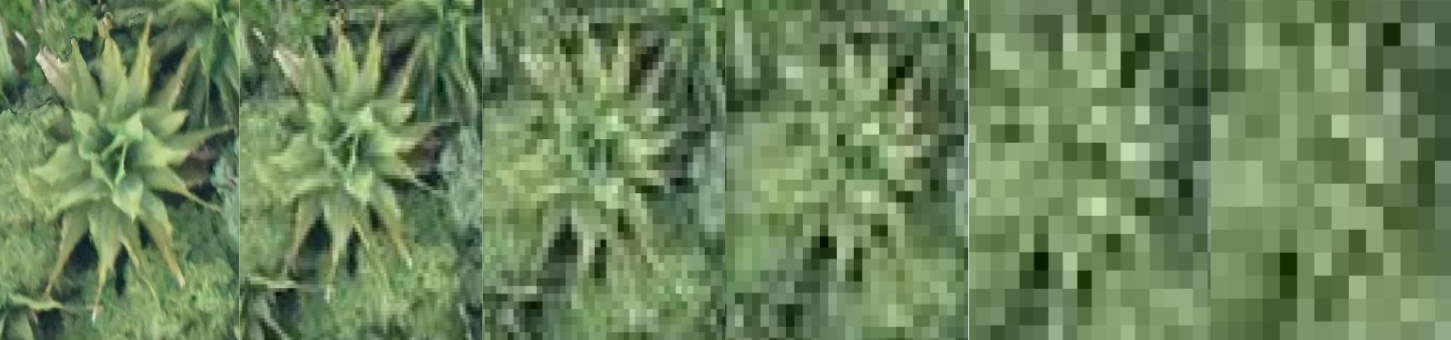
\includegraphics[width=1.0\textwidth]{Figures/Palm-resolution.png}
\caption{Resolution in cm/pixel from left to right: 5, 20, 40, 60, 80, 100. It is clear that after 60 cm/pixel the image becomes indiscernible.}
\label{fig:Palm-resolution}
\end{figure}

\subsection{Class Imbalance Issues}

Class imbalance played a large roll in our training. We found that training on both classes produced networks that could not localize deciduous trees at all. This is because the signal from Cohune Palm trees heavily out weights that of the deciduous trees during back-propagation. In the future we would like to explore weighting the loss function in order to place more emphasis on examples from classes with fewer instances.

\subsection{Ecological Impact}

We identified 6,308 palms at BFREE, yielding 120.4 ha palm coverage. Palms were more prevalent at BFREE, (disturbed) with $21\%$ palm cover, compared to only $5.9\%$ and $2.0\%$ in our less-disturbed, mountain sites (BNR). Total palm coverage in the BNR ranged from 6.2 ha - 27.3 ha. Our preliminary data for deciduous trees at BFREE resulted in identifying 2,389 trees with a total coverage of 17.8 ha or $3.0\%$. Our results conform well with past on-the-ground data for both tree types. Cohune palms tend to grow in disturbed areas, but also contribute to soil organics. Deciduous tree crown area calculated in comparable rainforests ranged from $~3-10\%$. This study shows how UAV and CNNs can save time (vs. manual) identifying specific tree species, helping to determine key rainforest habitat characteristics, as well as aid research and management of remote areas.

\begin{figure}[ht]
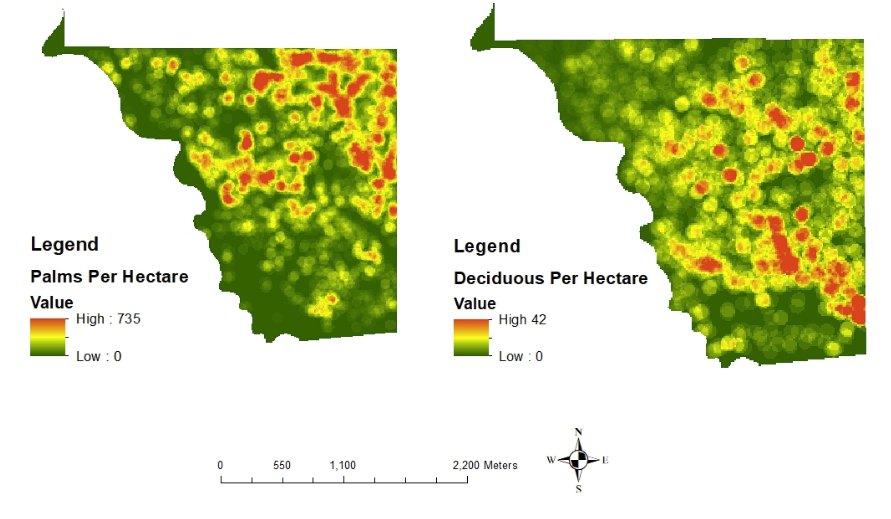
\includegraphics[width=1.0\textwidth]{Figures/HeatMaps.png}
\caption{Left: Cohune Palm Trees Right: Deciduous Trees. Note that the two classes of trees grow in distinct location from each other.}
\label{fig:HeatMaps}
\end{figure}
